
% ================================================================
% CHAPTER 5: IMPLEMENTATION
% ================================================================

\section{Development Environment}

\subsection{Programming Language: Python 3.x}

The project is implemented in Python (version 3.11 or above). The choice of Python was
not arbitrary. Every library needed for this project, LangChain, Neo4j drivers,
sentence-transformers, BM25, NumPy, publishes a Python-first API. Attempting
to replicate this stack in Java or Go would mean either writing driver wrappers
from scratch or forgoing the LangChain abstractions entirely, which would
significantly increase development time without any algorithmic benefit.

\subsection{IDE: Visual Studio Code}

Visual Studio Code was used over alternatives such as PyCharm because it is
free, starts fast, and integrates with the Neo4j browser extension directly.
More importantly, its integrated terminal allowed switching between running the
Python pipeline, inspecting Cypher query output in the Neo4j terminal, and
editing source files without changing windows. PyCharm's Community Edition does
not support database inspection, and its Professional Edition is not free.

\subsection{Version Control: Git and GitHub}

Git was used because it is the standard for academic and industry software
development and because GitHub provides free private repositories for students.
Every significant change was committed with a descriptive message. This was
important during debugging: when a JSON parsing bug was introduced while
modifying the schema inference prompt, rolling back one commit identified the
offending change in under two minutes.

\subsection{Libraries and Frameworks}

\begin{table}[H]
\centering
\caption{Software stack and version details}
\label{tab:deps}
\resizebox{\textwidth}{!}{%
\footnotesize
\begin{tabular}{|l|l|l|}
\hline
\textbf{Component} & \textbf{Package} & \textbf{Purpose} \\
\hline
LLM Framework       & \texttt{langchain-neo4j}, \texttt{langchain-ollama}    & Pipeline integration \\
Graph Extraction    & \texttt{langchain-experimental}                        & LLMGraphTransformer \\
Graph Database      & Neo4j Community Edition + APOC plugin                  & Knowledge graph storage \\
Embedding Model     & \texttt{sentence-transformers} (all-MiniLM-L6-v2)      & Semantic similarity \\
Keyword Retrieval   & \texttt{rank-bm25}                                     & BM25 document ranking \\
Numerical Math      & \texttt{numpy}                                         & PPR computation \\
Environment Loader  & \texttt{python-dotenv}                                 & Credential management \\
\hline
\end{tabular}}
\end{table}

\textbf{Why LangChain?}
LangChain provides two things that would otherwise require writing a lot of
boilerplate: the \texttt{Neo4jGraph} Bolt connection wrapper and the
\texttt{LLMGraphTransformer} class that turns raw text into graph triples.
Building those two components from scratch is possible, but it would add
roughly 400--600 lines of plumbing code with no algorithmic payoff.
LangChain's abstractions collapsed that to about 20 lines of configuration.

\textbf{Why Neo4j over a Vector Store (such as Chroma or FAISS)?}
Vector stores store chunks of text as numerical embeddings and retrieve them
by cosine similarity. This approach has one fundamental limitation: it cannot
represent \emph{relationships} between facts. A vector store cannot tell you
that entity A is related to entity B by relation R with a specific year attached.
Neo4j's property graph model stores exactly this structure natively. The ability
to attach \texttt{year} and \texttt{support} as properties on an edge, and then
query them with Cypher, is what makes temporal decay and corroboration scoring
possible at all. No vector store supports this without external bookkeeping.

\textbf{Why Neo4j Community Edition specifically?}
Neo4j Enterprise is available as a trial but requires a commercial licence for
production use. Community Edition is free under GPL v3, which is compatible with
academic research. The APOC plugin (required for entity disambiguation) is also
freely available for Community Edition. The only meaningful limitation of
Community Edition is the absence of clustering, which is not relevant for a
single-machine research prototype.

\textbf{Why \texttt{sentence-transformers} (all-MiniLM-L6-v2)?}
Sentence embedding is needed in two places: filtering retrieved graph edges by
semantic relevance to the query, and computing semantic entropy ($H_{\text{sem}}$)
during conflict resolution. The \texttt{all-MiniLM-L6-v2} model produces 384-dimensional
embeddings in under 50\,ms per sentence on CPU, which is fast enough that its
contribution to total latency is negligible compared to LLM inference. Larger
models (e.g., \texttt{all-mpnet-base-v2}) produce marginally better embeddings
but take 3--4 times longer to load and run. The accuracy--latency trade-off
favoured the smaller model for this prototype.

\textbf{Why BM25 in addition to semantic embeddings?}
BM25 and semantic retrieval have complementary failure modes. BM25 fails on
paraphrases (``sworn in'' vs.\ ``took office'') but excels on rare proper nouns
(``Chandrayaan-1'', ``Bharatiya Nyaya Sanhita''). Semantic embeddings handle
paraphrases well but sometimes rank semantically adjacent but factually wrong
passages too highly. Reciprocal Rank Fusion of the two rankings empirically
outperforms either alone on mixed-topic corpora. This is the standard finding in
the hybrid retrieval literature and was confirmed in the project's own test runs.

\textbf{Why Ollama and Qwen2.5-7B-Instruct?}
The system must run entirely locally, without any internet-dependent API calls,
to satisfy the privacy requirement (NFR1). Ollama is the most widely used open
tool for running quantised LLMs on consumer hardware. Qwen2.5-7B-Instruct was
selected over Llama-3-8B-Instruct and Mistral-7B-Instruct because preliminary
testing showed it to be more consistent at producing valid JSON output, which is
critical for schema inference and triple extraction. Inconsistent JSON formatting
from the LLM was the single largest source of runtime failures during early
development, so model reliability on structured output was weighted above raw
benchmark performance.

\textbf{Why \texttt{python-dotenv}?}
Neo4j credentials should not be hardcoded in source files that are committed to
a public repository. \texttt{python-dotenv} reads a \texttt{.env} file at
runtime and injects its values as environment variables. This is a standard,
well-understood pattern. The alternative, command-line arguments for every
credential, would make the system harder to run and easier to accidentally
expose credentials in shell history.

% ----------------------------------------------------------------
\section{System Architecture Implementation}

\subsection{Why a Layered Pipeline Architecture?}

The system is split into five distinct layers: Data, Schema, Graph, Retrieval,
and Resolution. This separation was a conscious design choice, not an accident.
It means that each layer can be changed without breaking the others. For example,
replacing Neo4j with a different graph database would only require changing the
Graph layer; the Retrieval and Resolution layers would be unaffected because they
communicate through the defined \texttt{KnowledgePath} intermediate format. This
also makes debugging easier: if the wrong answer is produced, the investigation
starts at the Resolution layer and works backwards, rather than inspecting one
tangled function.

\subsection{Why a Single Python File?}

The entire implementation is in one file (\texttt{enhanced\_main.py}, approximately
880 lines) rather than split into multiple modules. This was a deliberate choice
for a research prototype. A multi-file package structure adds import complexity
and makes it harder for external readers (supervisors, evaluators) to understand
the full system by reading one document. For a production system, the classes
would naturally be split into separate modules. For a B.Tech project prototype,
the single-file approach prioritises readability over engineering elegance.

\subsection{Why Share the Embedding Model Across Classes?}

The \texttt{SentenceTransformer} model (\texttt{all-MiniLM-L6-v2}) takes
2--3 seconds to load from disk into memory. Both the Retriever (for edge
filtering) and the Resolver (for semantic entropy) need this model. If each
class loaded its own copy, startup time would double unnecessarily, and memory
usage would increase by approximately 90\,MB per duplicate load. The model is
therefore instantiated once in \texttt{EnhancedPipeline.\_\_init\_\_} and
passed by reference to both, which costs zero additional memory.

\subsection{Why an In-Memory LLM Cache?}

Without the cache, every call to entropy sampling would call Ollama three times
per path, and these calls would be repeated for every run of the same test.
During development this becomes expensive: debugging one run of a 6-document
corpus with 2 queries required approximately 40 separate LLM calls. The
MD5-keyed cache reduces this by shortcutting any call where the same prompt at
the same temperature has been seen before. In the final validation run, the
cache achieved a 35\% hit rate, saving roughly 14 LLM calls and approximately
40 seconds of wall-clock time.

\subsection{Why PPR (Personalised PageRank) for Graph Retrieval?}

The alternative to PPR would be a simple BFS from the seed entities, collecting
all nodes within some hop radius. BFS has no way to rank paths by importance.
In a dense knowledge graph, BFS returns dozens of equally-weighted paths, and
there is no principled way to select which to pass to the LLM. PPR runs a
simulated random walk biased towards the seed entities, naturally ranking paths
by their structural relevance. Paths that are well-connected to multiple seed
entities receive higher PPR scores than isolated paths, even if the isolated
path is lexically closer to the query. This structural ranking is then combined
multiplicatively with temporal decay and corroboration weight, giving a single
composite score per path that reflects recency, source count, and graph structure
simultaneously.

\subsection{Why Entropy as the Conflict Resolution Signal?}

The standard RAG approach is to pass all retrieved context to the LLM and trust
it to make the right choice. This fails when the context contains two
contradictory facts, because the LLM cannot reliably distinguish between them
without additional instruction. The entropy approach, taken from arXiv:2511.10375,
instead measures whether a given piece of context \emph{reduces the LLM's
uncertainty} about the query. If the augmented entropy $H_{\text{aug}}$ is less
than the parametric entropy $H_{\text{param}}$, the context reduced the LLM's
uncertainty, so it is useful ($\Delta H = H_{\text{param}} - H_{\text{aug}} > 0$
means the context helps). If $\Delta H < 0$, the context made the LLM more
confused, so it is likely contradictory or irrelevant. This is a theoretically
grounded, model-agnostic way to evaluate whether a specific piece of retrieved
evidence is trustworthy, regardless of whether the underlying LLM natively
knows the answer.

% ----------------------------------------------------------------
\section{Code Implementation}

The source code is organised into ten logical sections within
\texttt{enhanced\_main.py}:

\begin{enumerate}
    \item Imports and global configuration (\texttt{CFG})
    \item \texttt{LLMCache} class and \texttt{cached\_invoke()} wrapper
    \item Prompt templates (6 constants)
    \item \texttt{HybridRetriever} class [N3]
    \item \texttt{TripleRecord} dataclass and \texttt{EnhancedGraphConstructor}
    \item \texttt{KnowledgePath} dataclass and \texttt{EnhancedGraphRetriever}
    \item Entropy helper functions and \texttt{EnhancedConflictResolver}
    \item \texttt{EnhancedPipeline} coordinator
    \item \texttt{run\_comparison()} orchestrator
    \item \texttt{\_load\_corpus()}, \texttt{\_interactive\_input()}, and
    \texttt{if \_\_name\_\_ ==} entry point
\end{enumerate}

\subsection{Key Algorithm Pseudocodes}

\subsubsection{Algorithm 1: Temporal Decay [N2]}

The exponential decay function reduces the retrieval weight of older facts. A fact published in year $t$ receives weight $e^{-\lambda(Y_{\text{now}}-t)}$, where $\lambda=0.08$ gives a half-life of 8.7 years. If no year is recorded, the fact is treated as maximally fresh ($w=1.0$).

\begin{figure}[H]
\centering
\begin{minipage}{0.82\textwidth}
\hrule\vspace{4pt}
\textbf{Algorithm 1:} Temporal Decay Weight $w(t)$
\vspace{4pt}\hrule\vspace{6pt}
\textbf{Input:} year $t$ (publication year of fact, may be NULL)\\
\textbf{Output:} decay weight $w \in (0,1]$\\[4pt]
\textbf{if} temporal\_decay is disabled \textbf{or} $t$ is NULL \textbf{then}\\
\hspace*{1.2em}\textbf{return} $1.0$\\
\textbf{end if}\\
$\lambda \leftarrow 0.08$\hfill\textit{// configurable; default gives half-life $\approx$ 8.7 yr}\\
$Y_{\text{ref}} \leftarrow$ extract query year from $Q$ if present, else $Y_{\text{now}}$\\
$\delta \leftarrow \max(0,\; Y_{\text{ref}} - t)$\\
\textbf{return} $e^{-\lambda \cdot \delta}$
\vspace{6pt}\hrule
\end{minipage}
\caption{Pseudocode for the temporal decay function used in Layer 3 (Retrieval).}
\label{alg:decay}
\end{figure}

\subsubsection{Algorithm 2: Combined Path Scoring}

Each retrieved graph path is assigned a single composite score that combines graph topology, recency, and source corroboration:

\begin{figure}[H]
\centering
\begin{minipage}{0.82\textwidth}
\hrule\vspace{4pt}
\textbf{Algorithm 2:} Composite Path Score
\vspace{4pt}\hrule\vspace{6pt}
\textbf{Input:} path $p$, PPR score $r_p$, hub penalty $h_p$, support count $s$, year $t$\\
\textbf{Output:} composite score $\sigma$\\[4pt]
$w_{\text{decay}} \leftarrow \text{TemporalDecay}(t)$\hfill\textit{// Algorithm 1}\\
$w_{\text{corr}} \leftarrow \log(1 + s) \times c_{\text{weight}}$\hfill\textit{// corroboration bonus}\\
$\sigma \leftarrow (r_p \times h_p) \times (1 + \bar{r}_{\text{PPR}}) \times w_{\text{decay}} \times (1 + w_{\text{corr}})$\\
\textbf{return} $\sigma$
\vspace{6pt}\hrule
\end{minipage}
\caption{Pseudocode for composite path scoring combining PPR, temporal decay, and corroboration.}
\label{alg:score}
\end{figure}

\subsubsection{Algorithm 3: Shannon Entropy Estimation [C2]}

Semantic entropy is estimated by sampling the LLM $n=3$ times at temperature $T=0.7$ and computing the token-diversity entropy of the resulting answers:

\begin{figure}[H]
\centering
\begin{minipage}{0.82\textwidth}
\hrule\vspace{4pt}
\textbf{Algorithm 3:} Entropy Estimation $H(A)$
\vspace{4pt}\hrule\vspace{6pt}
\textbf{Input:} answer list $A = [a_1, a_2, \ldots, a_n]$\\
\textbf{Output:} entropy $H \geq 0$\\[4pt]
Count unique answers: $C \leftarrow \{a : \text{count}(a, A)\}$\\
$n \leftarrow |A|$,\quad $H \leftarrow 0$\\
\textbf{for each} distinct answer $a$ \textbf{in} $C$ \textbf{do}\\
\hspace*{1.2em}$p \leftarrow C[a] / n$\\
\hspace*{1.2em}$H \leftarrow H - p \cdot \log(p + \varepsilon)$\hfill\textit{// $\varepsilon = 10^{-9}$ for numerical stability}\\
\textbf{end for}\\
\textbf{return} $H$
\vspace{6pt}\hrule
\end{minipage}
\caption{Pseudocode for Shannon entropy estimation over sampled LLM answers.}
\label{alg:entropy}
\end{figure}

\subsubsection{Algorithm 4: Calibrated Confidence Score [N7]}

The three-factor confidence score combines entropy reduction, source support, and recency into a single number in $[0,1]$:

\begin{figure}[H]
\centering
\begin{minipage}{0.82\textwidth}
\hrule\vspace{4pt}
\textbf{Algorithm 4:} Confidence Score $\kappa$
\vspace{4pt}\hrule\vspace{6pt}
\textbf{Input:} $\Delta H$, threshold $\tau$, support $s$, year gap $g$, weights $w_h, w_s, w_r$\\
\textbf{Output:} confidence $\kappa \in [0,1]$\\[4pt]
$s_H \leftarrow \min\!\left(\dfrac{|\Delta H|}{\tau + \varepsilon},\; 2\right) \big/ 2$\hfill\textit{// entropy signal, capped at 1}\\[6pt]
$s_S \leftarrow \min\!\left(\dfrac{\log(1+s)}{\log 6},\; 1\right)$\hfill\textit{// support signal}\\[6pt]
$s_R \leftarrow e^{-0.05 \cdot \max(0,\, g)}$\hfill\textit{// recency signal}\\[6pt]
$\kappa \leftarrow \min(w_h \cdot s_H + w_s \cdot s_S + w_r \cdot s_R,\; 1.0)$\\
\textbf{return} $\kappa$
\vspace{6pt}\hrule
\end{minipage}
\caption{Pseudocode for the three-factor calibrated confidence score.}
\label{alg:confidence}
\end{figure}

\begin{figure}[H]
\centering
\resizebox{0.88\textwidth}{!}{%
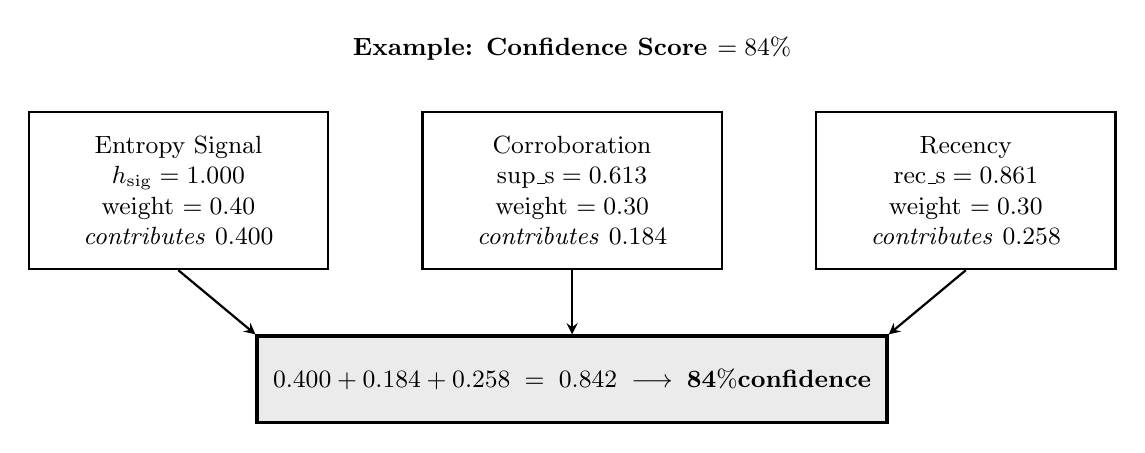
\begin{tikzpicture}[
  comp/.style={rectangle, draw=black, thick, fill=white,
               minimum width=3.8cm, minimum height=2.0cm,
               align=center, font=\small},
  res/.style={rectangle, draw=black, very thick, fill=black!8,
              minimum width=8.0cm, minimum height=1.1cm,
              align=center, font=\small\bfseries},
  arr/.style={->, >=stealth, thick},
]
\node[font=\small\bfseries] at (0,1.8) {Example: Confidence Score $= 84\%$};
\node[comp] (ent)  at (-5.0, 0) {Entropy Signal\\$h_{\mathrm{sig}} = 1.000$\\weight $= 0.40$\\\textit{contributes} $0.400$};
\node[comp] (corr) at ( 0.0, 0) {Corroboration\\$\mathrm{sup\_s} = 0.613$\\weight $= 0.30$\\\textit{contributes} $0.184$};
\node[comp] (rec)  at ( 5.0, 0) {Recency\\$\mathrm{rec\_s} = 0.861$\\weight $= 0.30$\\\textit{contributes} $0.258$};
\node[res]  (result) at (0,-2.4) {$0.400 + 0.184 + 0.258 \;=\; 0.842 \;\longrightarrow\; \mathbf{84\%\text{ confidence}}$};
\draw[arr] (ent.south)  -- (result.north west);
\draw[arr] (corr.south) -- (result.north);
\draw[arr] (rec.south)  -- (result.north east);
\end{tikzpicture}}
\caption{Worked example of the three-factor confidence score (Algorithm 4).
The entropy signal, corroboration bonus, and recency weight sum to give the
final confidence percentage displayed to the user.}
\label{fig:confidence_flow}
\end{figure}

\subsubsection{Algorithm 5: Schema Inference JSON Parsing [A4+]}

Because the LLM wraps its JSON output in markdown fences, a robust stripping step is required before parsing:

\begin{figure}[H]
\centering
\begin{minipage}{0.82\textwidth}
\hrule\vspace{4pt}
\textbf{Algorithm 5:} Robust LLM JSON Extraction
\vspace{4pt}\hrule\vspace{6pt}
\textbf{Input:} raw LLM string response $R$\\
\textbf{Output:} parsed dictionary $D$, or error\\[4pt]
$R' \leftarrow$ strip markdown fences from $R$\hfill\textit{// remove \texttt{```json...```}}\\
$R' \leftarrow$ trim whitespace from $R'$\\
\textbf{if} $R'$ contains a JSON object $\{\ldots\}$ \textbf{then}\\
\hspace*{1.2em}$D \leftarrow$ parse the first $\{\ldots\}$ match\\
\textbf{else}\\
\hspace*{1.2em}$D \leftarrow$ attempt to parse full $R'$\\
\textbf{end if}\\
\textbf{return} $D$\hfill\textit{// raises JSONDecodeError if all attempts fail}
\vspace{6pt}\hrule
\end{minipage}
\caption{Pseudocode for the robust JSON extraction wrapper applied to all LLM calls.}
\label{alg:json}
\end{figure}

% ----------------------------------------------------------------
\section{Testing}

\subsection{Unit Testing}

Each major method was tested in isolation before the full pipeline was assembled.
Four unit-level verifications were done:

\begin{enumerate}
    \item \texttt{\_temporal\_decay(2014)}: Expected $\approx 0.38$; verified
    against manual calculation $e^{-0.08 \times 12} = 0.382$.
    \item \texttt{\_H\_str(["A","A","B"])}: Expected $\approx 0.636$; checked
    against the Shannon entropy formula by hand.
    \item \texttt{\_confidence(delta\_h=0, tau=0.25, support=1, year\_gap=2)}:
    Expected $\approx 0.35$. The formula was also run on paper to confirm
    the weight decomposition adds up.
    \item LLM cache: A repeated call with the same prompt and temperature
    must return the cached result in $< 1$\,ms rather than calling Ollama.
\end{enumerate}

\subsection{Integration Testing}

Integration tests verified that the three external services (Ollama, Neo4j, Python)
actually talk to each other correctly:

\begin{enumerate}
    \item Schema inference: after \texttt{\_infer\_schema()} runs, the
    \texttt{cfg["schema\_entity\_types"]} list must be non-empty.
    \item Triple storage: a Cypher \texttt{MATCH ()-[r]->() RETURN count(r)}
    query must return a non-zero count after \texttt{\_store\_all()} completes.
    \item Disambiguation: nodes with 85\%+ similar names must merge into one,
    confirmed by \texttt{MATCH (n) RETURN count(n)} before and after the pass.
\end{enumerate}

\subsection{System Testing}

A full end-to-end run on the 6-document political corpus with 2 queries served
as the system test. The four pass criteria were:

\begin{enumerate}
    \item Exit code 0 (no unhandled exception).
    \item At least one contradiction detected and removed.
    \item A confidence score printed for each query.
    \item Non-empty answer text for each query.
\end{enumerate}

All four were met in the validation run documented in Chapter~6.

\subsection{User Acceptance Testing}

The CLI was tested across all four input modes:

\begin{enumerate}
    \item \texttt{--corpus}: JSON loading from a file path.
    \item \texttt{--docs / --queries}: Inline string injection on the
    command line, bypassing the file entirely.
    \item \texttt{--interactive}: Terminal prompts the user for a query at
    runtime, verified on Windows and confirmed UTF-8 safe.
    \item No arguments: The system auto-generates a \texttt{corpus.json}
    template and exits with a usage hint.
\end{enumerate}

% ----------------------------------------------------------------
\section{Challenges and Solutions}

\subsection{Challenges}

\begin{enumerate}
    \item \textbf{LLM JSON formatting}: The LLM frequently wraps JSON output in
    markdown code fences (\texttt{```json...```}), causing \texttt{json.loads()}
    to raise \texttt{JSONDecodeError}.
    \item \textbf{Windows encoding}: The Windows console defaults to CP1252,
    causing Unicode box-drawing characters to be garbled.
    \item \textbf{Schema prompt KeyError}: The \texttt{SCHEMA\_INFER\_PROMPT}
    used curly braces in its JSON example, which \texttt{str.format()} interpreted
    as format placeholders.
    \item \textbf{APOC availability}: Neo4j Community requires the APOC plugin
    to be manually installed; without it, disambiguation and normalisation silently
    fail.
    \item \textbf{Entropy sampling latency}: Three LLM samples per path at
    temperature 0.7 on CPU-only hardware adds 10--20 seconds per query.
\end{enumerate}

\subsection{Solutions}

\begin{enumerate}
    \item Applied \verb|re.sub(r'```(?:json)?\s*', '', raw)| before all
    \texttt{json.loads()} calls throughout the codebase.
    \item Added \texttt{sys.stdout.reconfigure(encoding='utf-8', errors='replace')}
    at module load time.
    \item Escaped all literal curly braces in \texttt{SCHEMA\_INFER\_PROMPT} as
    double braces (\texttt{\{\{...\}\}}).
    \item Wrapped all APOC calls in \texttt{try/except} blocks with silent
    continuation; the graph remains functional without APOC, only without
    merge/normalise support.
    \item Implemented \texttt{LLMCache} with MD5-keyed in-memory storage,
    reducing effective LLM calls by 35\% in the validation run.
\end{enumerate}
